\documentclass{article}
\usepackage{geometry}
\geometry{
 a4paper,
 left=30mm,
 top=30mm,
 }
 
\usepackage{graphicx}
\usepackage{caption}
\usepackage{subcaption}

\usepackage[utf8]{inputenc}
\usepackage{graphicx}
\graphicspath{ {images/} }
\usepackage{float, amsmath}
\usepackage{amsfonts}
\usepackage{graphicx}
\usepackage[
pdftitle={\WorkTitle},
pdfauthor={\FirstandFamilyName},
bookmarks=true,
colorlinks=true,
breaklinks=true,
urlcolor=brown,
citecolor=blue,
linkcolor=blue,
unicode=true,
]
{hyperref}
\usepackage{array,booktabs,makecell}

\newcommand{\searchGold}{\textit{searchGold }}
\newcommand{\stopp}{\textit{stop }}
\newcommand{\toDepot}{\textit{toDepot }}
\newcommand{\waiting}{\textit{waiting }}
\newcommand{\toHelp}{\textit{toHelp }}
\newcommand{\picking}{\textit{picking }}

\title{
World development indicators and Fragile States Index\\
\large Semester Project on course "Statistical methods in economics"\\
Teacher: PhDr. Mgr. Sherzod Tashpulatov}
\author{Galina Alperovich, shchegal@fel.cvut.cz}
\date{June, 2017}


\begin{document}
\maketitle
\tableofcontents
\bibliographystyle{abbrv}

\newpage
\section{Introduction}
% You introduce from which area of economics your research is about? For example, is it education economics or labor economics? You also provide an explanation why your research could be important and interesting.
In the current project, we consider macroeconomics World development indicators, which presents current and accurate global development data, and includes national, regional and global estimates \cite{WDI_site}. The World Development Indicators (WDI) might be categorized under different topics such as Economy & Growth, Social Development, Environment and so one.  We will choose 17 the most important indicators from each category, perform their analysis and use them as explanatory variables for the Fragile States Index (FSI). \\

FSI is another global indicator which was developed by Fund for Peace organization, and aim to reflect the state vulnerability to conflict. This index is based on comprehensive social science approach named Conflict Assessment System Tool (CAST). This approach includes analysis of publicly available data, news, and experts opinion \cite{FSI}.\\

All visualization and calculation will be made in statistical program Gretl \cite{Gretl}.


\section{Data description}
% Here you list all variables and their description. You also need to provide at least two types of plots: 1) histogram (comment if your distribution plot is symmetric or asymmetric),
% 2) x y scatter plot (comment if the trend is increasing or decreasing).
In this section, we list analyzed variables, their description and perform visualization. All listed indicators are taken for the 2010 year for the list of 177 countries with available information on indicators.\\

The list of variables is the following:

\begin{itemize}
  \item \textit{Fragile States Index} reflects the state vulnerability to conflict or collapse. We will use FSI as a dependent variable in our analysis. FSI equals to the sum of its 12 components. See the list of components on the table \ref{table:components}. We will not use them in the analysis, but it is important to understand from what factors FSI consists.
  \item We selected 20 the most valuable WDIs from every category based on Investopedia article \cite{WDI_important}. We use them as explanatory variables.
\end{itemize}

See the detailed list of variables in the table \ref{table:ind}.\\

By definition, the higher FSI for a country, the more vulnerability to conflict it has. To understand the shape of FSI distribution, let's draw the histogram and boxplot graphs. On the figure \ref{fig:fsi_hist} we see that the FSI distribution is asymmetric and has negative skewness. We can see the same pattern on the boxplot \ref{fig:fsi_box}. The mass of the distribution is concentrated on the right of the figure, what means the majority of the countries has relatively high FSI. On the left side of the distribution, we see the small peak around 30, developed countries such as the USA, Canada, Austria, France, Germany, etc. Northern countries such as Norway, Finland, Sweden, Ireland have the lowest FSI. African countries such as Somalia, Sudan, Zimbabwe have the highest FSI. \\

\begin{table}[h]
\begin{center}
{\renewcommand{\arraystretch}{1.2}
\begin{tabular}{lrrrrll}
\toprule
\textbf{Explanatory variables: World development indicators} &  \\
\midrule
GDP growth	&	\\
Employment rate	&	\\
Access to the water &	\\
Real interest rate	&	\\
Energy use	&	\\
Death rate	&	\\
Internet users	&	\\
Net flows on external debt	&	\\
Total tax rate (\% of commercial profits)	&	\\
Number of infants death	&	\\
Access to electricity (\% of population)	&	\\
Imports of goods and services (\% of GDP)	&	\\
Urban population (\% of total)	&	\\
School enrollment, primary (\% gross)	&	\\
Improved sanitation facilities (\% of population with access)	&	\\
Taxes on income, profits and capital gains & \\
Number of scientific articles	&	\\
\midrule
\textbf{Dependent variable: Fragile States Index}	&	\\
\bottomrule
\end{tabular}}
\caption{List of variables considered in the project. The data is taken for 177 countries in 2010.}
\label{table:ind}
\end{center}
\end{table} 

\begin{table}[h]
\begin{center}
{\renewcommand{\arraystretch}{1.2}
\begin{tabular}{lrrrrll}
\toprule
Security Apparatus	&	External Intervention\\
Factionalized Elites	&	Refugees and IDPs\\
Group Grievance	&	Demographic Pressures\\
Economic Decline	&	Human Rights and Rule of Law\\
Uneven Economic Development	& Public Services	\\
Human Flight and Brain Drain & State Legitimacy	\\
\bottomrule
\end{tabular}}
\caption{The list of 12 components of Fragile State Index which is calculated as their sum.}
\label{table:components}
\end{center}
\end{table} 

On the table \ref{table:sum_fsi} you can find the summary statistics for FSI. The coefficient of skewness is -0.56726. Originally for several indicators, we had missing values, so we performed missing values imputations with the corresponding mean of the variable. So now the number of missing values is zero.\\

\begin{table}[h]
\begin{center}
\begin{tabular}{lr}
\toprule
Mean  &                         71.874\\
Median  &                       77.100\\
Minimum &                      18.700\\
Maximum &                      114.30\\
Standard deviation  &           23.151\\
C.V.  &                        0.32210\\
Skewness            &       -0.56726\\
Ex. kurtosis    &               -0.46150\\
5\% percentile &                27.290\\
95\% percentile  &               105.14\\
Interquartile range &          30.400\\
Missing obs.  &                      0\\
\bottomrule
\end{tabular}
\caption{Summary statistics for Fragile States Index (177 observations)}
\label{table:sum_fsi}
\end{center}
\end{table}

\begin{figure}[h]
\begin{subfigure}{.5\textwidth}
  \centering
  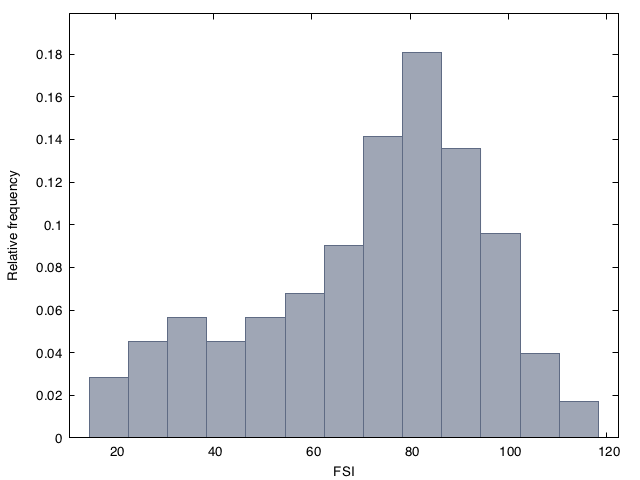
\includegraphics[width=1.0\textwidth]{fsi_histogram}
    \caption{Histogram of the FSI. The higher FSI, the more state vulnerability to conflict.}
    \label{fig:fsi_hist}
\end{subfigure} 
\begin{subfigure}{.5\textwidth}
  \centering
  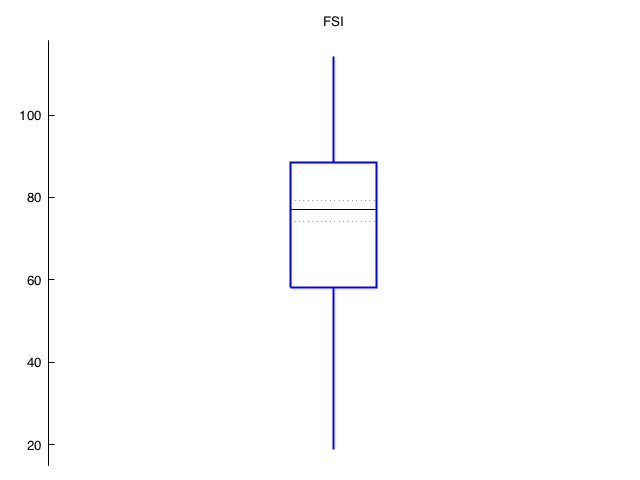
\includegraphics[width=1.0\textwidth]{fsi_boxplot}
    \caption{Boxplot of the FSI}
    \label{fig:fsi_box}
\end{subfigure}
\caption{Fragile States Index distribution}
\label{fig:fsi}
\end{figure}

Also, let's look at the relationship between some explanatory variable and the target variable FSI. After we had calculated correlations between FSI and all other variables, we found out that The number of Internet users indicator has the lowest negative correlation, what means, the more Internet users the country has, the lower FSI index. It's quite interesting observations, let's draw the scatter plot between these two variables, see figure \ref{fig:fsi_internet}. On the picture, we clearly observe negative linear dependence between these two variables. It is important to mention, that correlation does not mean causality, and thus we can state only that these two variables are changing linearly at the same time, but we don't know what variable influences on this change. The correlation matrix visualization can be found on the figure \ref{fig:corr}. 

\begin{figure}[H]
\begin{center}
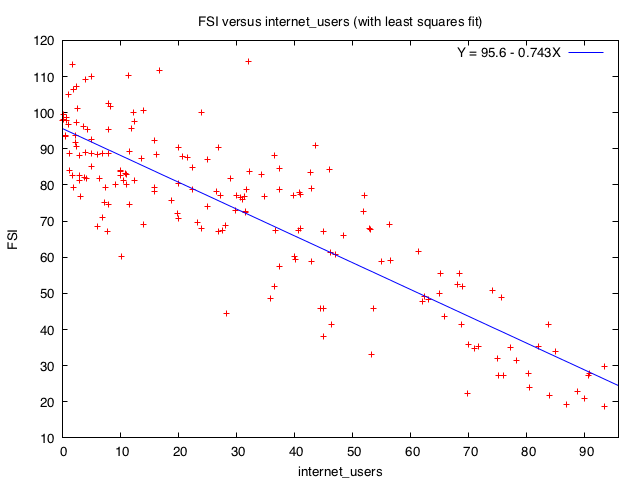
\includegraphics[width=.8\textwidth]{fsi_internet}
\caption{Linear relationship between the number of Internet users and FSI. We see negative linear dependence.}
\label{fig:fsi_internet}
\end{center}
\end{figure}

\begin{figure}[H]
\begin{center}
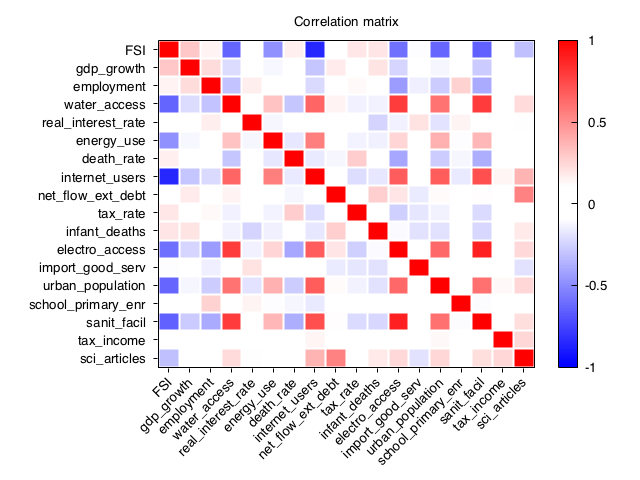
\includegraphics[width=1\textwidth]{corr}
\caption{Visualization of the correlation matrix between all variables. 5\% critical value (two-tailed test) = 0.1476}
\label{fig:corr}
\end{center}
\end{figure}

\section{Economic relationship}

On the figure \ref{fig:corr} we see the visualization of the correlation matrix. Red color means positive correlation; blue color means negative correlation. FSI is our target variable, so let's firstly analyze the apparent relationship between it and other variables. As we already mentioned, it has the lowest negative correlation with the number of Internet users. Also, FSI has such relationship with the following indicators: Water access, Energy use, Electricity access, Urban population and Sanitation facilities. This negative linear relationship reflects the main problems of the least developed countries: few people have access to the pure water, electricity and surely Internet. People mostly live not in the cities, and with the poor sanitation conditions. The FSI index can be considered also as a composite measure of country development. Also, we can see the high positive correlation between pairs of listed indicators.\\

Let's calculate the Variance Inflation Factor (VIF) for every explanatory variable. VIF provides an index that measures how much the variance of an estimated regression coefficient is increased because of collinearity. The values greater than 10.0 may indicate a collinearity problem. With Gretl, we calculated all VIFs and found out that all values are less than 7, what means we don't have multicollinearity problem and don't need to exclude variables. See the table \ref{table:vif}.


\begin{table}[H]
\begin{center}
\begin{tabular}{lr}
\toprule
        gdp\_growth  &   1.342 \\
        employment  &   1.650 \\
      water\_access  &   3.309 \\
real\_interest\_rate  &   1.321 \\
        energy\_use  &   1.737 \\
        death\_rate  &   1.485 \\
    internet\_users  &   4.431 \\
 net\_flow\_ext\_debt  &   1.752 \\
          tax\_rate  &   1.227 \\
     infant\_deaths  &   1.403 \\
    electro\_access  &   6.904 \\
  import\_good\_serv  &   1.298 \\
  urban\_population  &   2.364 \\
school\_primary\_enr  &   1.235 \\
       sanit\_facil  &   6.364 \\
        tax\_income  &   1.115 \\
      sci\_articles  &   2.038 \\
\bottomrule
\end{tabular}
\caption{Variance Inflation Factors for all explanatory variables. All values are less than 10 what means we don't have multicolleniarity problem.}
\label{table:vif}
\end{center}
\end{table}

% Here you specify dependent and explanatory variables. Also you provide a correlation matrix including p-values. Avoid multicollinearity problem among your explanatory variables.

\section{Methodology}
In this section, we will build the models for FSI based on selected WDIs. \\
\subsection{OLS}
Let's build the first Ordinary Least Squares model, and include all variables. See the table \ref{table:ols}. The quality of the model can be judged by $R^2$ coefficient, in our case it equals to 0.79, what is the relatively good but not he best quality. The p-value for each term in the table tests the null hypothesis that the regression coefficient is equal to zero (no effect). A low p-value ($<$ 0.05) indicates that you can reject the null hypothesis. In such way, we have four significant variables: Employment rate, Water access, Internet users and Urban population. \\

The standard assumption in linear regression is that the theoretical residuals are independent and normally distributed. Observed residuals are an estimate of the theoretical residuals, so let's test them on normality with QQ plot, see the figure \ref{fig:resid_qq}.  We see it is close to normal distribution (diagonal line), hence normality assumption holds. Also normality test with gives us the p-value = 0.740798, what means we can't reject null hypothesis about normality.\\

$$H_0: \text{errors are normally distributed}$$
$$H_1: \text{errors are not normally distributed}$$

\begin{figure}[H]
\begin{center}
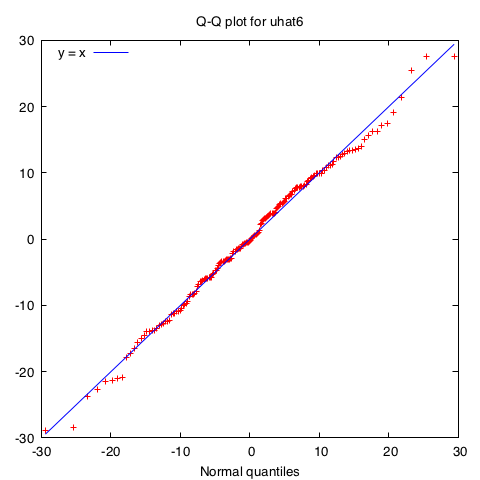
\includegraphics[width=.5\textwidth]{resid_qq}
\caption{QQ plot for residuals of the OLS model. We see it is close to normal distribution, hence normality assumption holds.}
\label{fig:resid_qq}
\end{center}
\end{figure}

\begin{table}[H]
\begin{center}
\begin{tabular}{lr@{.}lr@{.}lr@{.}lr@{.}l}
\toprule
  &
 \multicolumn{2}{c}{Coefficient} &
  \multicolumn{2}{c}{Std.\ Error} &
   \multicolumn{2}{c}{$t$-ratio} &
    \multicolumn{2}{c}{p-value} \\[1ex]
\toprule
const &
  147&089 &
    12&4407 &
      11&82 &
        0&0000 ***\\
gdp\_growth &
  0&294608 &
    0&266989 &
      1&103 &
        0&2715 \\
employment &
  $-$0&202418 &
    0&0923576 &
      $-$2&192 &
        0&0299 **\\
water\_access &
  $-$0&222474 &
    0&0968161 &
      $-$2&298 &
        0&0229 **\\
real\_interest\_rate &
  $-$0&0680424 &
    0&135074 &
      $-$0&5037 &
        0&6151 \\
energy\_use &
  $-$4&10924\textrm{e--05} &
    0&000427028 &
      $-$0&09623 &
        0&9235 \\
death\_rate &
  $-$0&258066 &
    0&303401 &
      $-$0&8506 &
        0&3963 \\
internet\_users &
  $-$0&592710 &
    0&0658440 &
      $-$9&002 &
        0&0000 ***\\
net\_flow\_ext\_debt &
  1&44676\textrm{e--10} &
    8&88111\textrm{e--11} &
      1&629 &
        0&1053 \\
tax\_rate &
  0&00134957 &
    0&0265030 &
      0&05092 &
        0&9595 \\
infant\_deaths &
  $-$4&19536\textrm{e--06} &
    9&43917\textrm{e--06} &
      $-$0&4445 &
        0&6573 \\
electro\_access &
  0&0289993 &
    0&0694400 &
      0&4176 &
        0&6768 \\
import\_good\_serv &
  $-$0&0446160 &
    0&0424610 &
      $-$1&051 &
        0&2950 \\
urban\_population &
  $-$0&127797 &
    0&0569667 &
      $-$2&243 &
        0&0263 **\\
school\_primary\_enr &
  $-$0&138846 &
    0&0862127 &
      $-$1&611 &
        0&1093 \\
sanit\_facil &
  $-$0&0347277 &
    0&0712599 &
      $-$0&4873 &
        0&6267 \\
tax\_income &
  1&56924\textrm{e--13} &
    1&47843\textrm{e--13} &
      1&061 &
        0&2901 \\
sci\_articles &
  $-$0&000163556 &
    0&000126628 &
      $-$1&292 &
        0&1984 \\
\toprule
\end{tabular}
\begin{tabular}{lrlr}
Mean dependent var &  71.87401 & S.D. dependent var &  23.15073 \\
Sum squared resid &  19901.63 & S.E. of regression &  11.18783 \\
$R^2$ &  0.789017 & Adjusted $R^2$ &  0.766460 \\
$F(17, 159)$ &  34.97747 & P-value($F$) &  6.18\textrm{e--45} \\
Log-likelihood & $-$669.0852 & Akaike criterion &  1374.170 \\
Schwarz criterion &  1431.341 & Hannan--Quinn &  1397.357 \\
\toprule
\end{tabular}
\end{center}
\caption{First OLS model for FSI, all linear terms are included. We can see a lot of insignificant variables.}
\label{table:ols}
\end{table}

\subsection{RESET test}
Now let's run the Ramsey’s RESET test for the first model specification. RESET test considers the following hypothesis:

$$H_0: \text{model is correctly specified}$$
$$H_1: \text{model is incorrectly specified}$$

For this test, we have p-value = 0.00133 what means we should reject the null hypothesis about the correctness of the model. It shows us that some components of the model might be included not in the linear form but quadratic or even cubic form. Let's build Auxiliary regression for RESET specification test to find quadratic components. In this regression, coefficient next to the quadratic terms is tested for equality to zero. See results on the table \ref{table:reset}. After this test, we will select the most significant quadratic variables to add them to the next model. The list of quadratic terms includes GDP growth, Employment rate, Water access, Death rate, Internet users, Net flows on external debt, Imported goods and services, Urban population and School enrollment. The list of the most significant linear terms from the original OLS model includes Employment rate, Water access, Internet users,  Urban population. We run the RESET test for cubic terms as well and found out that the Water access and Internet users are also can be added to the model in cubic form. \\

\begin{table}[H]
\begin{center}
\begin{tabular}{lrrrl}
\toprule
& coefficient & std. error  & t-ratio & p-value \\
\toprule
const & 315.013 & 50.9679 & 6.181 & 5.22e-09 *** \\
gdp\_growth & 0.747051  & 0.290985  & 2.567 & 0.0112 ** \\
employment  & −0.449082 & 0.115297  & −3.895  & 0.0001 *** \\
water\_access & −0.621257 & 0.150413  & −4.130  & 5.85e-05 *** \\
real\_interest\_ra~ & −0.167452 & 0.134069  & −1.249  & 0.2135  \\
energy\_use & 0.000222429 & 0.000420831 & 0.5285  & 0.5979 \\
death\_rate & −0.671893 & 0.318191  & −2.112  & 0.0363 ** \\
internet\_users & −1.28433  & 0.213706  & −6.010  & 1.24e-08 *** \\
net\_flow\_ext\_debt  & 2.51920e-10 & 9.16473e-11 & 2.749 & 0.0067 *** \\
tax\_rate & 0.00842815  & 0.0257539 & 0.3273  & 0.7439 \\
infant\_deaths  & −6.88892e-06  & 9.17664e-06 & −0.7507 & 0.4539  \\
electro\_access & 0.0412992 & 0.0673531 & 0.6132  & 0.5406 \\
import\_good\_serv  & −0.0824425  & 0.0426113 & −1.935  & 0.0548 * \\
urban\_population & −0.295141 & 0.0740259 & −3.987  & 0.0001 *** \\
school\_primary\_e~ & −0.390419 & 0.111700  & −3.495  & 0.0006 *** \\
sanit\_facil  & −0.111289 & 0.0726174 & −1.533  & 0.1274 \\
tax\_income & 2.84887e-13 & 1.48081e-13 & 1.924 & 0.0562 * \\
sci\_articles & −0.000217790  & 0.000123682 & −1.761  & 0.0802 * \\
\toprule
\end{tabular}
\end{center}
\caption{Auxiliary regression for RESET specification test, quadratic terms.}
\label{table:reset}
\end{table}


\subsection{Final OLS model}
Let's build a new OLS model with the linear, quadratic and cubic terms. See the results for the model on the table \ref{table:ols2}. As we can see we included the following variables: squared School enrollment, squared Internet users, cubic Water access and Urban population. We reduced the number of variables from 17 to 4 without loss of quality (we got $R^2$ even a bit higher). After collinearity check, we could observe that all VIF values are less than 3, what means we don't have collinearity problem.\\

\begin{table}[h]
\begin{center}
\vspace{1em}
\begin{tabular}{lr@{.}lr@{.}lr@{.}lr@{.}l}
\toprule
  &
 \multicolumn{2}{c}{Coefficient} &
  \multicolumn{2}{c}{Std.\ Error} &
   \multicolumn{2}{c}{$t$-ratio} &
    \multicolumn{2}{c}{p-value} \\[1ex]
\toprule
const &
  111&153 &
    4&77485 &
      23&28 &
        0&0000 ***\\
school\_primary\_enr\_2 &
  $-$0&000747504 &
    0&000347218 &
      $-$2&153 &
        0&0327 **\\
internet\_users\_2 &
  $-$0&00665839 &
    0&000475151 &
      $-$14&01 &
        0&0000 ***\\
water\_access\_3 &
  $-$2&05824\textrm{e--05} &
    3&77392\textrm{e--06} &
      $-$5&454 &
        0&0000 ***\\
urban\_population &
  $-$0&0852354 &
    0&0482812 &
      $-$1&765 &
        0&0793 *\\
\toprule
\end{tabular}

\vspace{1ex}
\begin{tabular}{lrlr}
\toprule
Mean dependent var &  71.87401 & S.D. dependent var &  23.15073 \\
Sum squared resid &  19178.76 & S.E. of regression &  10.55956 \\
$R^2$ &  0.796681 & Adjusted $R^2$ &  0.791953 \\
$F(4, 172)$ &  168.4902 & P-value($F$) &  2.22\textrm{e--58} \\
Log-likelihood & $-$665.8108 & Akaike criterion &  1341.622 \\
Schwarz criterion &  1357.502 & Hannan--Quinn &  1348.062 \\
\toprule
\end{tabular}
\end{center}

\caption{Final OLS model for FSI. Linear, quadratic and cubic terms are included. Number of variables is reduced from 17 to 4.}
\label{table:ols2}
\end{table}

\subsection{Heteroskedasticity test}

Let's run White's test for heteroskedasticity in order to check whether the variance of the errors in a regression model is constant. White's test considers the following hypothesis:

$$H_0: \text{homoskedasticity is presented}$$
$$H_1: \text{heteroskedasticity is presented}$$

We got the p-value = 0.223339, what means we don't reject null hypothesis and we deal with homoskedasticity case. 


% Lecture notes \cite{Lect}\\
% Based on the correlation analysis specify a multiple regression model. Your model should have at least two factors (i.e., explanatory variables).

\section{Estimation}

The final regression model is specified on the table \ref{table:ols2}. The equation of the model is the following:\\


\begin{gather}
\begin{split}
\widehat{\rm FSI} &= 
\underset{(23.279)}{111.153}
-\underset{(-2.153)}{0.000747504}\,\mbox{school\_primary\_enr\_2}
-\underset{(-14.013)}{0.00665839}\,\mbox{internet\_users\_2}\\
& -\underset{(-5.454)}{2.05824\textrm{e--05}}\,\mbox{water\_access\_3}
-\underset{(-1.765)}{0.0852354}\,\mbox{urban\_population}
\end{split}
 \notag \\
T = 177 \quad \bar{R}^2 = 0.7920 \quad F(4,172) = 168.49 \quad \hat{\sigma} = 10.560 \notag \\
\centerline{($t$-statistics in parentheses)} \notag
\end{gather}


Let's run the Ramsey’s RESET test for the final specification. RESET test considers the following hypothesis:

$$H_0: \text{model is correctly specified}$$
$$H_1: \text{model is incorrectly specified}$$

\noindent We see the following result:\\

\noindent RESET test for specification (squares and cubes)\\
Test statistic: F = 1.988712,\\
with p-value = P(F(2,167) $>$ 1.98871) = 0.14\\

\noindent RESET test for specification (squares only)\\
Test statistic: F = 0.257972,\\
with p-value = P(F(1,168) $>$ 0.257972) = 0.612\\

\noindent RESET test for specification (cubes only)\\
Test statistic: F = 0.009258,\\
with p-value = P(F(1,168) $>$ 0.00925784) = 0.923\\

We observe that all p-values are greater than 0.05, that means we don't reject the hypothesis about the correct specifications of the model. Hence the specification is correct.\\

Let's compare real target values and fitted values from the model. Firstly, look at the scatter plot composed of $FSI \text{ and } \widehat{FSI}$. On the figure \ref{fig:y_yhat} we can see that predictions are not perfect (all points are not on the same line) but it is close to the line. \\

Also we can calculate the following quality measures between $FSI \text{ and } \widehat{FSI}$:\\

\noindent Mean Error:                       -1.6619e-14 \\
Root Mean Squared Error:           10.31 \\
Mean Absolute Error:               8.1059\\
Mean Percentage Error:            -2.793\\
Mean Absolute Percentage Error:    13.424\\

As for a coefficient of determination $R^2$, we see the following result:\\

\noindent $R^2$ : 0.797 \\
$\text{Adjusted } R^2$ : 0.792 \\
p-value: 2.22e-58 refers to the testing of $R^2$ on equality to zero, it will be discussed later in the section \ref{good}.\\

\begin{figure}[h]
\begin{center}
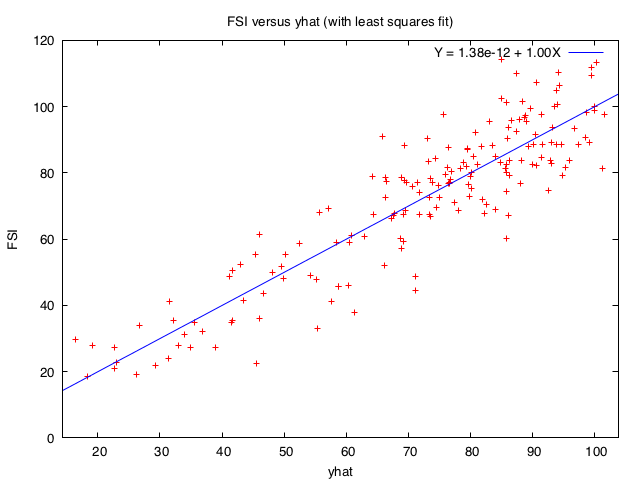
\includegraphics[width=.8\textwidth]{y_yhat}
\caption{Scatter plot between $FSI \text{ and } \widehat{FSI}$}
\label{fig:y_yhat}
\end{center}
\end{figure}

% Here you provide estimation results from Excel or EViews. Also conduct Ramsey’s RESET test for model specification (make sure to specify H0 and H1 in your project).
% For this purpose, you need to create and save the fitted values of y according to the model in H0.

\section{Statistical inference}
% Conduct hypothesis testing regarding the significance of estimated model parameters (make sure to specify H0 and H1 for each model parameter in your project).
To test the significance of every variable in the model we consider the following hypothesis for every coefficient corresponding to the explanatory variable:

$$H_0: \beta_j = 0, \text{for all } j$$
$$H_1: \beta_j > 0$$

All variables have p\_value $<$ 0.08 and hence significant result (reject null hypothesis). 

\section{Goodness of fit test}
\label{good}
% Conduct the significance test of the overall model (make sure to specify H0 and H1 in your project).
To test the significance of the overall model, we test the coefficient of determination $R^2$ which shows how much our model explains the changes in the dependent variable, by using independent variables \cite{Lect}. The test uses F-statistic and considers the following hypothesis:

$$H_0: R^2 = 0$$
$$H_1: R^2 > 0$$

In our case p-value = 2.22e-58 what means F-statistic is in the tail and our decision is rejecting $H_0$, hence $R^2$ is significant.

\section{Economic verification}
% Explain if the signs of estimated model parameters correspond to economic intuition.
All four included variables have a negative sign, what means we have negative linear relationship between these variables and the target FSI variable. We discussed this in the first section, where we looked at the correlation matrix. In that section, we also observed negative correlation coefficient.\\

In our case, the higher proportion of the children enrolled in the primary school, the lower FSI index (we remember, that Finland, Norway, and other north countries have the lowest FSI). The higher number of Internet users, Number of people with water access, Urban population, the lower FSI. 

\section{Interpretation}
% Provide an interpretation of the estimated parameters. Also provide an interpretation of the R-squared (coefficient of determination).

The $R^2$ coefficient of determination can be interpreted as follows: our four explanatory variables (plus the constant) explain 80\% of the variance of our dependent (target) variable FSI. \\

Interpretation of the coefficient can be as follows: 

$$ \frac{d(FSI)}{d(school\_primary\_enr)} = -2 \cdot 0.000747 \cdot mean(school\_primary\_enr) = -0,001495 \cdot 105.25 = -0,157$$

That means that if in average the proportion of children enrolled to the primary school increases by 1, the FSI index will decrease by 0.15. The same is actual for the other three variables: 

$$ \frac{d(FSI)}{d(internet\_users)} = -2 \cdot 0.00665839 \cdot mean(internet\_users) = 
-0.00665839 \cdot 32  = -0,21$$

$$ \frac{d(FSI)}{d(water\_access)} = -3 \cdot − 2.05824e–05 \cdot mean(water\_access)^2 = -2.05824e–05 \cdot 86.476 = -0,17$$

$$ \frac{d(FSI)}{d(urban\_population)} = - 0.0852354$$

Hence, if in the average proportion of the Internet users increases by 1, the FSI index will decrease by 0.21. If in the average proportion of the people who have access to the water increases by 1, the FSI index will decrease by 0.17. If the share of Urban population increases by 1, the FSI index will decrease by 0.08.

\section{Conclusion}
% Here you need to summarize the major finding and conclusion of your project.
In this project, we analyzed various global World development indicators for 177 countries for the 2010 year. We considered 17 the most important indicators from different categories and analyzed how they influence on the Fragile State Index. We discovered that there are four the most significant indicators which explain 80\% of FSI variance: Proportion of the children enrolled in the primary school, Number of Internet users, Proportion of the people with access to the water and Urban population. The interesting fact is that the Number of Internet users and FSI has the lowest negative correlation among other variables, and hence the negative linear relationship. The simplest linear regression model with only this one variable explains 74\% of FSI variance, and thus this indicator is the most significant for FSI prediction.\\

We performed missing values imputation, correlation analysis, we built a linear regression model for FSI based on various WDIs, checked collinearity and heteroskedasticity and also run RESET test to find quadratic and cubic components for the model. \\

FSI is calculated by the independent company Fund for Peace and requires a lot of expertise and comprehensive analysis. In this project, we showed that it is possible to built statistical model for FSI based on only four publicly available WDI variables which explain 80\% of FSI changes. In further works, it would be a good direction to consider other 970 different WDIs and build a more complicated model to improve the prediction of FSI.

\bibliography{reference}



\end{document}




